\section{Out-of-sample tests}\label{app:sealed}

Every frozen policy tested out of sample keeps its change rate's 95\% upper bound below 5\% under our parsers (all eleven tests: Figure~\ref{fig:oos}, Tables~\ref{tab:e2e} and~\ref{tab:holdout}). Each ran once, with routes and outputs saved before gold labels were decoded. Only the large-pair ARC and SQuAD tests are sealed, and MMLU-Pro has no unused questions. These runs are not a second calibration. The sealed and held-out protocols define no pass rule, whereas the later ones do. The contamination caveat of Appendix~\ref{app:restson} applies.

\begin{figure}[!t]\centering
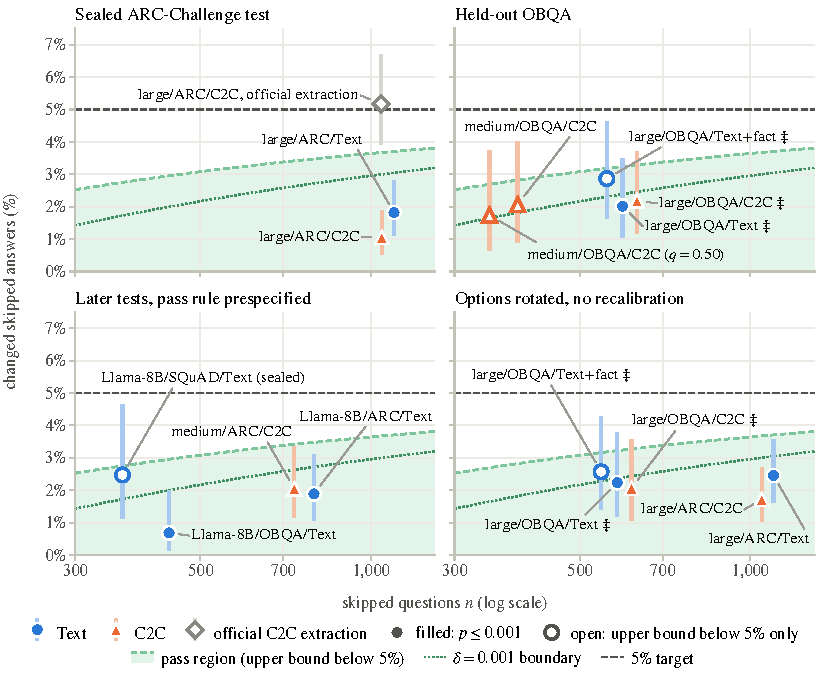
\includegraphics[width=\linewidth]{figures/figure_oos.pdf}
\caption{Every frozen policy tested out of sample keeps the 95\% upper bound of its change rate below 5\% under our parsers; only the sealed C2C policy read with the official C2C extraction exceeds it. Each marker is one frozen run on questions its pair had not used (official extraction: the sealed C2C run re-read), placed at its number of skipped questions $n$ (log scale) and the share of skipped answers that change, with its two-sided 95\% Clopper--Pearson interval as a vertical line; the counts are in the tables below. Shaded region under the dashed curve: rates whose upper bound is below 5\% at that $n$ (pass rule: a 95\% upper bound below 5\%); dotted curve: the largest rate at which the test rejects $\rho\ge0.05$ at $\delta=0.001$; dashed horizontal line: the 5\% target. Filled: the test rejects at $\delta=0.001$; open: only the upper bound is below 5\% (level 0.025). Official C2C extraction (gray diamond): the official C2C evaluator's answer extraction applied to the stored outputs. $q=0.50$: sensitivity threshold for medium/OBQA/C2C (deployed $q=0.55$). Options rotated: each option's text moved one position down, labels kept. $^\ddagger$: nominal development certificate (Appendix~\ref{app:history}). Where a Text and a C2C run share $n$, the C2C marker is drawn slightly to the right. The rotated runs set no pass rule, and their p-values are descriptive. Every statistic is in Tables~\ref{tab:e2e}, \ref{tab:holdout}, \ref{tab:oos_later}, and~\ref{tab:rotation} and Appendices~\ref{app:sealed} and~\ref{app:squad}.}
\label{fig:oos}
\end{figure}

\paragraph{Sealed ARC test.} The population is all 1,172 ARC-Challenge test rows of \texttt{allenai/ai2\_arc} (1,172 groups after frozen normalization), with none removed. The sealing order was: (1) a freeze recorded that the test population had not been accessed and sealed the protocol, configuration, source index, and analysis snapshot; (2) only the \texttt{id}, \texttt{question}, and \texttt{choices} were projected; (3) after all scores, routes, outputs, probe records, and timings were written, a second freeze locked them; (4) only then was the answer key decoded. The thresholds are the development ones ($q=0.95$ and $0.90$), and no test quantile was computed. The four paths (fixed Text, Text policy, fixed C2C, C2C policy) were interleaved in one allocation, completing all 4,688 requests and 2,344 probes. The two policies' independent probes had identical inputs and scores. All 197 reference-routed outputs match the fixed-reference path, and \textsc{invalid} counts were 0/0 (Text) and 1/1 (C2C). The Text and C2C policies change 20 of 1,100 and 11 of 1,047 skipped answers ([1.11\%, 2.79\%] and [0.53\%, 1.87\%]; 1.71 and 0.94\% of all questions). Relative to the reference, they gain 7 and lose 12 correct answers (Text), and gain 7 and lose 3 (C2C). The probe costs 42.5 and 40.5~ms (accuracy and latency: Table~\ref{tab:e2e_full}). On questions below the frozen thresholds, the sealed split does not significantly differ from the training split (Fisher $p=0.65$ and $0.68$). Its change rates are no higher than on development (Text 1.8 vs.\ 3.2\%, C2C 1.05 vs.\ 1.11\%).

\paragraph{Sealed ARC under the official extraction.} Under a rule fixed before computing, we re-read the stored sealed outputs using the official C2C extraction on the 1,169 questions lacking a fifth option (both policies skip the other three, none of which changes under our parser). Two unparseable answers count as agreement; counting them as changes leaves every count unchanged. The Text policy is unaffected (20 of 1,097 skipped answers change under both extractions, 1.82\% [1.12, 2.80]). However, 54 of 1,044 skipped C2C answers change (5.17\% [3.91, 6.70]; $p=0.635$), against 11 under our parser. Labels differ on 44 skipped questions, accounting for all 43 additional changes. A mechanical audit, fixed before computing, found that each of these 44 outputs starts with a single option letter followed by that option's own text, contains no second option label, and receives that letter from our parser. The official extraction marks every one unparseable because the option text contains a string treated as a math term (\texttt{tan} in 17, a minus sign in 10, \texttt{sin} in 7, a plus sign or slash in 4 each, \texttt{cos} in 3, and \texttt{mod} in 2; some contain two). The Text policies remain nearly unaffected elsewhere: on the held-out OBQA questions, the official extraction changes 11 of 595 skipped large-pair Text answers (1.85\% [0.93, 3.28], against 12 under our parser) and 16 of 558 Text+fact answers, matching our parser. As fixed in advance for a point estimate above 5\%, we state that the sealed C2C result holds under our parser only. The official C2C release includes an ARC test configuration, but we could not verify whether its fusers were exposed to these questions.

\paragraph{Held-out OBQA.} These are the 744 OBQA questions that the project's partition never assigned to fit, calibration, or development. The protocol's gate initially stopped the run because an earlier project stage had generated small-pair outputs on them under four communication channels and scored them against the answer key. Before any output existed, the protocol was amended to report them as held out rather than sealed, after two checks verified that no output, score, route, or latency of the medium or large pair existed for these questions, and that no artifact of this study reads the earlier stage's predictions or scores (two aggregate small-pair accuracies and two rows of the earlier scoring were read during the gate check, as the amendment, fixed before the run, discloses). Only \texttt{id}, \texttt{question}, and \texttt{choices} (plus \texttt{fact1} for Text+fact) were projected. Saved fit rows were reproduced bit for bit, and one shard was rerun after a bookkeeping failure that produced no output. With no pass rule set, all five upper bounds fall below 5\% (level 0.025). Only large Text and C2C (two nominal settings) also reject at $\delta=0.001$ ($p=1.5\times10^{-4}$ and $3.7\times10^{-4}$; with Bonferroni over the five tests, their family level is 0.005). Text+fact, also nominal, rejects only at 0.025. Always skipping would change 8.2 to 17.5\% of answers (Table~\ref{tab:holdout}). The two medium thresholds reach identical accuracy: of the 42 questions whose skip status differs, only two have an answer that C2C would change, and these cancel out. No latency was measured.

\begin{table}[!htbp]\centering\scriptsize
\caption{All five held-out OBQA tests keep the 95\% upper bound below 5\%, and large Text and C2C also reject at $\delta=0.001$ (744 questions). Change rate with its two-sided Clopper--Pearson 95\% CI; $p$: single prespecified test of $H_0:\rho\ge 0.05$; Level: stricter level at which $H_0$ is rejected (0.025: upper end below 5\%); Always skip: change rate of answering alone; (b) accuracy of the policy and the fixed reference, and their difference $\Delta$acc with its paired-bootstrap 95\% CI; pp: percentage points. The medium $q=0.50$ row is a sensitivity threshold (deployed $q=0.55$).}
\label{tab:holdout}
\renewcommand{\arraystretch}{1.1}\setlength{\tabcolsep}{3pt}
\vspace{5pt}\textit{(a) Changed answers}\par\smallskip
\begin{tabular*}{\linewidth}{@{}l@{\hspace{5pt}\extracolsep{\fill}}ccccc@{}}\toprule
Policy & \begin{tabular}[b]{@{}c@{}}Changed\\/ skipped\end{tabular} & \begin{tabular}[b]{@{}c@{}}Change rate (\%)\\{}[95\% CI]\end{tabular} & $p$ & Level & \begin{tabular}[b]{@{}c@{}}Always\\skip (\%)\end{tabular}\\\midrule
medium/OBQA/C2C, $q=0.55$ & 8/388 & 2.06 [0.89, 4.02] & $2.5\times10^{-3}$ & 0.025 & 17.47\\
medium/OBQA/C2C, $q=0.50$ & 6/346 & 1.73 [0.64, 3.74] & $1.4\times10^{-3}$ & 0.025 & 17.47\\
large/OBQA/Text, $q=0.80$ & 12/595 & 2.02 [1.05, 3.50] & $1.5\times10^{-4}$ & 0.001 & 8.20\\
large/OBQA/C2C, $q=0.80$ & 13/595 & 2.18 [1.17, 3.71] & $3.7\times10^{-4}$ & 0.001 & 8.33\\
large/OBQA/Text+fact, $q=0.75$ & 16/558 & 2.87 [1.65, 4.61] & $9.2\times10^{-3}$ & 0.025 & 11.02\\\bottomrule
\end{tabular*}
\par\vspace{17pt}
\textit{(b) Accuracy}\par\smallskip
\begin{tabular*}{\linewidth}{@{}l@{\hspace{5pt}\extracolsep{\fill}}cccc@{}}\toprule
& \multicolumn{2}{c}{Accuracy (\%)} & \multicolumn{2}{c}{$\Delta$acc, policy $-$ reference (pp)}\\\cmidrule(lr){2-3}\cmidrule(l){4-5}
Policy & Policy & Reference & & 95\% CI\\\midrule
medium/OBQA/C2C, $q=0.55$ & 61.16 & 60.89 & $+0.27$ & [$-0.54$, $+1.08$]\\
medium/OBQA/C2C, $q=0.50$ & 61.16 & 60.89 & $+0.27$ & [$-0.40$, $+0.94$]\\
large/OBQA/Text, $q=0.80$ & 86.02 & 86.96 & $-0.94$ & [$-1.88$, $-0.13$]\\
large/OBQA/C2C, $q=0.80$ & 81.45 & 80.24 & $+1.21$ & [$+0.40$, $+2.15$]\\
large/OBQA/Text+fact, $q=0.75$ & 89.65 & 91.13 & $-1.48$ & [$-2.55$, $-0.54$]\\\bottomrule
\end{tabular*}
\end{table}

\paragraph{Later out-of-sample tests.} The two Llama-8B policies (using the large pair's stored helper messages) and medium/ARC/C2C ran once on questions their respective pairs had never seen. They ran under a protocol fixed before any output, whose pass rule was a 95\% upper bound below 5\%. Before the runs, a gate confirmed that no output of the Llama-3.1-8B receiver or the medium pair's models existed for them. All three pass and reject at 0.001, with coverage within 1.2 points of development (Table~\ref{tab:oos_later}). This holds under the official extraction too (3 of 440, 15 of 792, and 16 of 730 changes on the A--D questions). One analysis run stopped after writing the seal receipts, so only the gold stage was recomputed from the sealed route files. The SQuAD test is in Appendix~\ref{app:squad}.

\begin{table}[!htbp]\centering\scriptsize
\caption{All three later out-of-sample tests pass their prespecified rule and reject at 0.001, with test coverage within 1.2 points of development coverage. Pass rule: a 95\% upper bound below 5\%. ARC test: held out for these pairs (Table~\ref{tab:e2e}). Change rate with its Clopper--Pearson 95\% CI; $p$: exact-test p-value; always skip: disagreement over the whole population; (b) accuracy in percent and $\Delta$acc, policy minus reference, with its paired-bootstrap 95\% CI; pp: percentage points.}
\label{tab:oos_later}
\renewcommand{\arraystretch}{1.1}\setlength{\tabcolsep}{2.5pt}
\vspace{5pt}\textit{(a) Changed answers}\par\smallskip
\begin{tabular*}{\linewidth}{@{}l@{\hspace{5pt}\extracolsep{\fill}}ccccccc@{}}\toprule
& & \multicolumn{2}{c}{Coverage (\%)} & & & & \\\cmidrule(lr){3-4}
Policy & \begin{tabular}[b]{@{}c@{}}Test\\questions\end{tabular} & Test & \begin{tabular}[b]{@{}c@{}}Develop-\\ment\end{tabular} & \begin{tabular}[b]{@{}c@{}}Changed\\/ skipped\end{tabular} & \begin{tabular}[b]{@{}c@{}}Change rate (\%)\\{}[95\% CI]\end{tabular} & $p$ & \begin{tabular}[b]{@{}c@{}}Always\\skip (\%)\end{tabular}\\\midrule
Llama-8B/OBQA/Text, $q=0.60$ & held-out OBQA (744) & 59.1 & 59.0 & 3/440 & 0.68 [0.14, 1.98] & $3.7\times10^{-7}$ & 11.96\\
Llama-8B/ARC/Text, $q=0.70$ & ARC test (1,172) & 67.7 & 68.9 & 15/794 & 1.89 [1.06, 3.10] & $4.4\times10^{-6}$ & 10.75\\
medium/ARC/C2C, $q=0.60$ & ARC test (1,172) & 62.5 & 63.2 & 15/733 & 2.05 [1.15, 3.35] & $3.1\times10^{-5}$ & 14.85\\\bottomrule
\end{tabular*}
\par\vspace{17pt}
\textit{(b) Accuracy}\par\smallskip
\begin{tabular*}{\linewidth}{@{}l@{\hspace{5pt}\extracolsep{\fill}}ccccc@{}}\toprule
& \multicolumn{3}{c}{Accuracy (\%)} & \multicolumn{2}{c}{$\Delta$acc, policy $-$ reference (pp)}\\\cmidrule(lr){2-4}\cmidrule(l){5-6}
Policy & $R$ & Reference & Policy & & 95\% CI\\\midrule
Llama-8B/OBQA/Text, $q=0.60$ & 80.38 & 83.06 & 82.66 & $-0.40$ & [$-0.94$, 0.00]\\
Llama-8B/ARC/Text, $q=0.70$ & 81.31 & 84.73 & 84.56 & $-0.17$ & [$-0.77$, $+0.43$]\\
medium/ARC/C2C, $q=0.60$ & 75.94 & 72.18 & 72.53 & $+0.34$ & [$-0.26$, $+0.94$]\\\bottomrule
\end{tabular*}
\end{table}


\paragraph{Option rotation.} With every option's text moved one position down (labels in place, as in the null control of Appendix~\ref{app:complementarity}), the five frozen large-pair policies ran once on the sealed ARC and held-out OBQA questions. They ran under a protocol fixed before any rotated output, with no recalibration and no gold label read; all outputs were written before the protocol's cutoff. With the rotation set to the identity, the run reproduced the stored scores bit for bit and the stored outputs byte for byte on 16 questions per population. The rotation check included 28 ARC questions with numeric labels or other than four options. The policies skip 73.3 to 93.9\% of questions and change 1.7 to 2.6\% of skipped answers, and every 95\% upper bound stays below 5\% (Table~\ref{tab:rotation}). Receiver-only answers before and after rotation agree on 98.7\% (ARC) and 98.0\% (OBQA) of questions with $u=0$ in the original order, against 85.9 and 75.9\% for the others. Of the $u=0$ questions, 90.0 and 77.7\% keep $u=0$. References agree with their original-order answers on 79.2 to 95.7\% of questions, with 0 to 2 unparseable answers per arm. All 27 rotated ARC/Text changes fall on questions with $u>0$, as in the original order.

\begin{table}[!htbp]\centering\scriptsize
\caption{With the options rotated by one position, every frozen large-pair policy keeps its 95\% upper bound below 5\% (one run, no recalibration; 1,172 ARC and 744 OBQA questions). Option rotation: each option's text moved one position down, labels kept. $u=0$: share of questions after rotation. Changed at $u=0$, $u>0$: changes among skipped questions by their $u$ on the rotated input. Intervals: Clopper--Pearson 95\% CI. $p$: exact-test p-value, descriptive. Original order: changed and skipped answers without rotation (Tables~\ref{tab:e2e} and~\ref{tab:holdout}).}
\label{tab:rotation}
\renewcommand{\arraystretch}{1.1}\setlength{\tabcolsep}{2.5pt}
\begin{tabular*}{\linewidth}{@{}l@{\hspace{5pt}\extracolsep{\fill}}cccccccccc@{}}\toprule
& & & \multicolumn{2}{c}{Coverage (\%)} & & & & \multicolumn{2}{c}{Changed at} & \\\cmidrule(lr){4-5}\cmidrule(lr){9-10}
Policy & \begin{tabular}[b]{@{}c@{}}$u=0$\\(\%)\end{tabular} & Skipped & rotated & original & Changed & \begin{tabular}[b]{@{}c@{}}Change rate (\%)\\{}[95\% CI]\end{tabular} & $p$ & $u=0$ & $u>0$ & \begin{tabular}[b]{@{}c@{}}Original order:\\changed / skipped\end{tabular}\\\midrule
large/ARC/Text & 72.1 & 1,100 & 93.9 & 93.9 & 27 & 2.45 [1.62, 3.55] & $1.5\times10^{-5}$ & 0 & 27 & 20/1,100\\
large/ARC/C2C & 72.1 & 1,049 & 89.5 & 89.3 & 18 & 1.72 [1.02, 2.70] & $1.9\times10^{-8}$ & 3 & 15 & 11/1,047\\
large/OBQA/Text & 46.1 & 582 & 78.2 & 80.0 & 13 & 2.23 [1.19, 3.79] & $5.4\times10^{-4}$ & 1 & 12 & 12/595\\
large/OBQA/C2C & 46.1 & 582 & 78.2 & 80.0 & 12 & 2.06 [1.07, 3.57] & $2.2\times10^{-4}$ & 1 & 11 & 13/595\\
large/OBQA/Text+fact & 46.1 & 545 & 73.3 & 75.0 & 14 & 2.57 [1.41, 4.27] & $3.4\times10^{-3}$ & 2 & 12 & 16/558\\\bottomrule
\end{tabular*}
\end{table}


